
% This LaTeX was auto-generated from MATLAB code.
% To make changes, update the MATLAB code and republish this document.

\documentclass[oneside]{book}
\usepackage[margin=3.27cm, bindingoffset=0cm]{geometry}
\usepackage{graphicx}
\usepackage{color}
\usepackage{minted}
\usepackage[most]{tcolorbox}
\usepackage{booktabs}
\definecolor{lightgreen}{rgb}{0.56, 0.93, 0.56}
\definecolor{moonstoneblue}{rgb}{0.45, 0.66, 0.76}
\definecolor{grey}{rgb}{0.5, 0.5, 0.5}

\sloppy
\definecolor{lightgray}{gray}{0.5}
\setlength{\parindent}{0pt}

\begin{document}

\begin{center}
    {\huge \textbf{4DV117 - Applied Machine Learning Project}}
    % \break Submitted By:
\end{center}

% \begin{center}
% \section*{}
% \begin{tabular}[t]{c@{\extracolsep{8em}}c} 
% \textbf{Prasannjeet Singh}  & \textbf{Farah Naz} \\
% \textit{Software Developer} & \textit{Doctoral Student} \\ 
% \textit{IST Group AB} & \textit{Linköping University} \\
% Växjö, Sweden & Linköping, Sweden \\
% prasannjeet.singh@ist.com & farah.naz@liu.se \\
% ps222vt@student.lnu.se & fn222gm@student.lnu.se \\
% \end{tabular}
% \end{center}

\begin{par}
% Submitted by \textbf{Prasannjeet Singh} and \textbf{Farah Naz}
\end{par} \vspace{1em}
\begin{par}

\end{par} \vspace{1em}

\section*{Contents}

\begin{itemize}
\setlength{\itemsep}{-1ex}
   \item 1. Preprocessing the Dataset
   \item 2. Segregating Training and Testing Datasets
   \item 3. Linear Regression
   \item 4. K-Nearest Neighbor Classification
   \item 5. Error Correcting Output Code Model (ECOC)
   \item 6. Unsupervised Learning
   \item 7. Summary
\end{itemize}


\section*{1. Preprocessing the Dataset}

\begin{par}
The data consists of 34 columns, where two of them are ID and Actual Diagnosis. When importing the data, we don't really need ID column, as it assumed that it does not affect in the diagnosis. Thus that column will be removed. Furthermore the Diagnosis column will be moved to the last while importing the data.
\end{par} \vspace{1em}
\begin{par}
Also, we will set up the import options in such a way that any row containing empty items will be ignored while import.
\end{par} \vspace{1em}


\subsection*{About the Dataset:}

\begin{par}
The dataset consists of 10 different properties of a cell-nuclei image. These properties are recorded from three different angle of a three dimentional space. Hence, there are 30 features in this dataset. The 10 properties are:
\end{par} \vspace{1em}
\begin{enumerate}
\setlength{\itemsep}{-1ex}
   \item Radius (mean of distances from center to points on the perimeter)
   \item Texture (standard deviation of gray-scale values)
   \item Perimeter
   \item Area
   \item Smoothness (local variation in radius lengths)
   \item Compactness (perimeter\^{}2 / area - 1.0)
   \item Concavity (severity of concave portions of the contour)
   \item Concave points (number of concave portions of the contour)
   \item Symmetry
   \item Fractal dimension ("coastline approximation" - 1)
\end{enumerate}

\begin{tcolorbox}[
    enhanced,
    attach boxed title to top left={xshift=6mm,yshift=-2mm},
    colback=moonstoneblue!20,
    colframe=moonstoneblue,
    colbacktitle=moonstoneblue,
    title=MATLAB Code,
    fonttitle=\bfseries\color{black},
    boxed title style={size=small,colframe=moonstoneblue,sharp corners},
    sharp corners,
    text width=140mm
    ]
\begin{minted}[linenos]{matlab}
% Extracting the import options
opts = detectImportOptions('Data/wdbc.data', 'FileType', 'text');
% In the Import Options, changing the rule to omit all the rows if a cell
% has missing value
opts.MissingRule = 'omitrow';
% Also specifying the number of columns that we need to be imported.
opts.SelectedVariableNames = [3:32 2];
% Reading the table according to the import options we created above
inputData = readtable('Data/wdbc.data', opts);
% Now converting the input data into matrix
args = [table2array(inputData(:,1)), table2array(inputData(:, 2:end-1))];
sol = ((categorical(table2array(inputData(:,end)))) == 'M')*1;
data = [args sol]; clear args; clear sol;
\end{minted}
\end{tcolorbox}

\section*{2. Segregating Training and Testing Datasets}

\begin{par}
In this step, we'll keep 100 datasets for testing and the rest for training our machine learning model.
\end{par} \vspace{1em}

\begin{tcolorbox}[
    enhanced,
    attach boxed title to top left={xshift=6mm,yshift=-2mm},
    colback=moonstoneblue!20,
    colframe=moonstoneblue,
    colbacktitle=moonstoneblue,
    title=MATLAB Code,
    fonttitle=\bfseries\color{black},
    boxed title style={size=small,colframe=moonstoneblue,sharp corners},
    sharp corners,
    text width=140mm
    ]
\begin{minted}[linenos]{matlab}
originalData = data;
testData = data(end-100: end, :);
data(end-100:end, :) = [];
% Now dividing the training data into features and responses
features = data(:,1:end-1);
response = data(:,end);
\end{minted}
\end{tcolorbox}


\section*{3. Linear Regression}

\begin{par}
At the first step, we will apply linear regression to the model and compare the results
\end{par} 

\subsection*{Feature Selection}

\begin{par}

\end{par} \vspace{1em}
\begin{par}
We can use the method sequentialfs() for feature selection.
\end{par} \vspace{1em}

\begin{tcolorbox}[
    enhanced,
    attach boxed title to top left={xshift=6mm,yshift=-2mm},
    colback=moonstoneblue!20,
    colframe=moonstoneblue,
    colbacktitle=moonstoneblue,
    title=MATLAB Code,
    fonttitle=\bfseries\color{black},
    boxed title style={size=small,colframe=moonstoneblue,sharp corners},
    sharp corners,
    text width=140mm
    ]
\begin{minted}[linenos]{matlab}
rng('default') %so that result can be replicated
fun = @(XT,yT,Xt,yt)loss(fitclinear(XT, yT),Xt,yt);
opts = statset('Display','iter');
inmodel = sequentialfs(fun,features,response,'options',opts);
\end{minted}
\end{tcolorbox}

\begin{tcolorbox}[
    enhanced,
    attach boxed title to top left={xshift=6mm,yshift=-2mm},
    colback=black,
    colframe=grey,
    colbacktitle=grey,
    title=System Output,
    coltext=white,
    fonttitle=\bfseries\color{white},
    boxed title style={size=small,colframe=grey,sharp corners},
    sharp corners,
    text width=100mm,
]
\begin{minted}{text}

Start forward sequential feature selection:
Initial columns included:  none
Columns that can not be included:  none
Step 1, added column 21, criterion value 0.0017917
Step 2, added column 27, criterion value 0.00121527
Step 3, added column 22, criterion value 0.000918642
Step 4, added column 29, criterion value 0.000776115
Final columns included:  21 22 27 29 

\end{minted}
\end{tcolorbox}


\begin{par}
As it can be seen, the above function suggests to use the column 21,22, 27 and 29 for training. We can apply linear regression on both the complete dataset and the subset from feature selection, and test it on the test data to see the difference.
\end{par} 

\subsection*{Linear Regression Without Feature Selection}

\begin{par}

\end{par} \vspace{1em}

\begin{tcolorbox}[
    enhanced,
    attach boxed title to top left={xshift=6mm,yshift=-2mm},
    colback=moonstoneblue!20,
    colframe=moonstoneblue,
    colbacktitle=moonstoneblue,
    title=MATLAB Code,
    fonttitle=\bfseries\color{black},
    boxed title style={size=small,colframe=moonstoneblue,sharp corners},
    sharp corners,
    text width=140mm
    ]
\begin{minted}[linenos]{matlab}

% Applying linear regression for classification for complete data
linearModel = fitclinear(features, response);

% Now we have our linear model above. Let us now try to predict the
% responses from our test data and find out the accuracy.
predictedSolution = predict(linearModel, testData(:,1:end-1));
accuracy = sum((predictedSolution == testData(:,end))*1)...
    /size(testData,1)*100

\end{minted}
\end{tcolorbox}


\begin{tcolorbox}[
    enhanced,
    attach boxed title to top left={xshift=6mm,yshift=-2mm},
    colback=black,
    colframe=grey,
    colbacktitle=grey,
    title=System Output,
    coltext=white,
    fonttitle=\bfseries\color{white},
    boxed title style={size=small,colframe=grey,sharp corners},
    sharp corners,
    text width=100mm,
]
\begin{minted}{text}

accuracy =

   92.0792

\end{minted}
\end{tcolorbox}



\begin{par}
Above, first we compared the predicted solution with the actual solution to obtain a logical vector, which was then added to find out the total number of accurate response, after which the percentage was calculated with respect to the total number of input data (which is 101 in our case). Hence, we see that the accuracy percentage is 92.08\%.
\end{par} 

\subsection*{Linear Regression With Feature Selection}


\begin{par}

\end{par} \vspace{1em}
\begin{par}
Now we will only use the features suggested by feature selection and apply the same procedure:
\end{par} \vspace{1em}


\begin{tcolorbox}[
    enhanced,
    attach boxed title to top left={xshift=6mm,yshift=-2mm},
    colback=moonstoneblue!20,
    colframe=moonstoneblue,
    colbacktitle=moonstoneblue,
    title=MATLAB Code,
    fonttitle=\bfseries\color{black},
    boxed title style={size=small,colframe=moonstoneblue,sharp corners},
    sharp corners,
    text width=140mm
    ]
\begin{minted}[linenos]{matlab}

linearModelFS = fitclinear(features(:,[21,22,27,29]), response);
% Predicting the response and comparing it with the test data:
predictedSolution = predict(linearModelFS, testData(:, [21,22,27,29]));
accuracy = sum((predictedSolution == testData(:,end))*1)...
    /size(testData,1)*100

\end{minted}
\end{tcolorbox}


\begin{tcolorbox}[
    enhanced,
    attach boxed title to top left={xshift=6mm,yshift=-2mm},
    colback=black,
    colframe=grey,
    colbacktitle=grey,
    title=System Output,
    coltext=white,
    fonttitle=\bfseries\color{white},
    boxed title style={size=small,colframe=grey,sharp corners},
    sharp corners,
    text width=100mm,
]
\begin{minted}{text}

accuracy =

   97.0297

\end{minted}
\end{tcolorbox}


    \begin{par}
Here the same methodology was used to find out the accuracy. And as it turns out, the accuracy is significantly more when only the columns suggested by feature selection method is used. In this case the accuracy jumps to 97.03\%.
\end{par} 

\subsection*{K Fold Cross Validation}

\begin{par}

\end{par} \vspace{1em}
\begin{par}
Let us first try 10-Fold cross validation on the complete dataset: Here we will use the complete dataset, and not the test and training dataset.
\end{par} \vspace{1em}


\begin{tcolorbox}[
    enhanced,
    attach boxed title to top left={xshift=6mm,yshift=-2mm},
    colback=moonstoneblue!20,
    colframe=moonstoneblue,
    colbacktitle=moonstoneblue,
    title=MATLAB Code,
    fonttitle=\bfseries\color{black},
    boxed title style={size=small,colframe=moonstoneblue,sharp corners},
    sharp corners,
    text width=140mm
    ]
\begin{minted}[linenos]{matlab}

% Using the complete dataset:
features = originalData(:,1:end-1);
response = originalData(:,end);
% Applying 10-fold cross validation
indices = crossvalind('Kfold', response, 10);
cp = classperf(response);
for i = 1:10
    test = (indices == i);
    train = ~test;
    kFoldModel = fitclinear(features(train,:), ...
        response(train,:));
    class = predict(kFoldModel, features(test,:));
    classperf(cp, class, test);
end
cp.CorrectRate*100

\end{minted}
\end{tcolorbox}

\begin{tcolorbox}[
    enhanced,
    attach boxed title to top left={xshift=6mm,yshift=-2mm},
    colback=black,
    colframe=grey,
    colbacktitle=grey,
    title=System Output,
    coltext=white,
    fonttitle=\bfseries\color{white},
    boxed title style={size=small,colframe=grey,sharp corners},
    sharp corners,
    text width=100mm,
]
\begin{minted}{text}

ans =

   92.6186

\end{minted}
\end{tcolorbox}


    \begin{par}
As we can see in the 10-Fold cross validation above, the correct rate, i.e. the percentage of the ratio of the number of correctly classified samples and the total number of classified samples is 92.62\%, signifying a fairly good model.
\end{par} \vspace{1em}
\begin{par}
We can now try cross validation on only the columns suggested by the feature selection method.
\end{par} \vspace{1em}

\begin{tcolorbox}[
    enhanced,
    attach boxed title to top left={xshift=6mm,yshift=-2mm},
    colback=moonstoneblue!20,
    colframe=moonstoneblue,
    colbacktitle=moonstoneblue,
    title=MATLAB Code,
    fonttitle=\bfseries\color{black},
    boxed title style={size=small,colframe=moonstoneblue,sharp corners},
    sharp corners,
    text width=140mm
    ]
\begin{minted}[linenos]{matlab}

% Applying 10-fold cross validation
indices = crossvalind('Kfold', response, 10);
cp = classperf(response);
for i = 1:10
    test = (indices == i);
    train = ~test;
    kFoldModel = fitclinear(features(train,[21,22,27,29]), response(train,:));
    class = predict(kFoldModel, features(test,[21,22,27,29]));
    classperf(cp, class, test);
end
cp.CorrectRate*100

\end{minted}
\end{tcolorbox}

\begin{tcolorbox}[
    enhanced,
    attach boxed title to top left={xshift=6mm,yshift=-2mm},
    colback=black,
    colframe=grey,
    colbacktitle=grey,
    title=System Output,
    coltext=white,
    fonttitle=\bfseries\color{white},
    boxed title style={size=small,colframe=grey,sharp corners},
    sharp corners,
    text width=100mm,
]
\begin{minted}{text}

ans =

   95.6063

\end{minted}
\end{tcolorbox}


    \begin{par}
As we can see the success rate in this case has increased to 95.61\% which is in accordance with our previous findings where we segregated the dataset into test and training. This suggests that for linear regression, we get better results with using only the features suggested by the feature selection method.
\end{par} \vspace{1em}


\section*{4. K-Nearest Neighbor Classification}

\begin{par}
Here, we will perform the same steps like above using kNN Classification. Here we will use 5-nearest neighbors.
\end{par} \vspace{1em}

\begin{tcolorbox}[
    enhanced,
    attach boxed title to top left={xshift=6mm,yshift=-2mm},
    colback=moonstoneblue!20,
    colframe=moonstoneblue,
    colbacktitle=moonstoneblue,
    title=MATLAB Code,
    fonttitle=\bfseries\color{black},
    boxed title style={size=small,colframe=moonstoneblue,sharp corners},
    sharp corners,
    text width=140mm
    ]
\begin{minted}[linenos]{matlab}

% Resetting the features and response variables to represent only the
% training data
features = data(:,1:end-1);
response = data(:,end);

\end{minted}
\end{tcolorbox}


\begin{par}

\end{par} \vspace{1em}

\begin{tcolorbox}[
    enhanced,
    attach boxed title to top left={xshift=6mm,yshift=-2mm},
    colback=moonstoneblue!20,
    colframe=moonstoneblue,
    colbacktitle=moonstoneblue,
    title=MATLAB Code,
    fonttitle=\bfseries\color{black},
    boxed title style={size=small,colframe=moonstoneblue,sharp corners},
    sharp corners,
    text width=140mm
    ]
\begin{minted}[linenos]{matlab}

% Feature selection like previously done for kNN.
% Standardizing the noncategorical predictor data.
rng('default') %so that result can be replicated
fun = @(XT,yT,Xt,yt)loss(fitcknn(XT, yT...
    ,'NumNeighbors',5,'Standardize',1),Xt,yt);
opts = statset('Display','iter');
inmodel = sequentialfs(fun,features,response,'options',opts);

\end{minted}
\end{tcolorbox}


\begin{tcolorbox}[
    enhanced,
    attach boxed title to top left={xshift=6mm,yshift=-2mm},
    colback=black,
    colframe=grey,
    colbacktitle=grey,
    title=System Output,
    coltext=white,
    fonttitle=\bfseries\color{white},
    boxed title style={size=small,colframe=grey,sharp corners},
    sharp corners,
    text width=100mm,
]
\begin{minted}{text}

Start forward sequential feature selection:
Initial columns included:  none
Columns that can not be included:  none
Step 1, added column 8, criterion value 0.00187303
Step 2, added column 22, criterion value 0.00132308
Step 3, added column 14, criterion value 0.000767153
Final columns included:  8 14 22 
\end{minted}
\end{tcolorbox}

    \begin{par}
As we can see above, suggested column to use are 8, 22 and 14.
\end{par} 

\subsection*{kNN Without Feature Selection}

\begin{par}

\end{par} \vspace{1em}

\begin{tcolorbox}[
    enhanced,
    attach boxed title to top left={xshift=6mm,yshift=-2mm},
    colback=moonstoneblue!20,
    colframe=moonstoneblue,
    colbacktitle=moonstoneblue,
    title=MATLAB Code,
    fonttitle=\bfseries\color{black},
    boxed title style={size=small,colframe=moonstoneblue,sharp corners},
    sharp corners,
    text width=140mm
    ]
\begin{minted}[linenos]{matlab}
% Applying kNN for classification for complete data
knnModel = fitcknn(features, response,'NumNeighbors',5,'Standardize',1);

% Now we have our kNN model above. Let us now try to predict the
% responses from our test data and find out the accuracy.
predictedSolution = predict(knnModel, testData(:,1:end-1));
accuracy = sum((predictedSolution == testData(:,end))*1)/size(testData,1)*100
\end{minted}
\end{tcolorbox}

\begin{tcolorbox}[
    enhanced,
    attach boxed title to top left={xshift=6mm,yshift=-2mm},
    colback=black,
    colframe=grey,
    colbacktitle=grey,
    title=System Output,
    coltext=white,
    fonttitle=\bfseries\color{white},
    boxed title style={size=small,colframe=grey,sharp corners},
    sharp corners,
    text width=100mm,
]
\begin{minted}{text}

accuracy =

   96.0396

\end{minted}
\end{tcolorbox}


    \begin{par}
As it can be seen, the accuracy using kNN classification is 96.04\%
\end{par} 

\subsection*{Linear Regression With Feature Selection}

\begin{par}

\end{par} \vspace{1em}
\begin{par}
Now we will only use the features suggested by feature selection and apply the same procedure:
\end{par} \vspace{1em}


\begin{tcolorbox}[
    enhanced,
    attach boxed title to top left={xshift=6mm,yshift=-2mm},
    colback=moonstoneblue!20,
    colframe=moonstoneblue,
    colbacktitle=moonstoneblue,
    title=MATLAB Code,
    fonttitle=\bfseries\color{black},
    boxed title style={size=small,colframe=moonstoneblue,sharp corners},
    sharp corners,
    text width=140mm
    ]
\begin{minted}[linenos]{matlab}

kNNModelFS = fitcknn(features(:,[8,14,22]),response...
    ,'NumNeighbors',5,'Standardize',1);
% Predicting the response and comparing it with the test data:
predictedSolution = predict(kNNModelFS, testData(:,[8,14,22]));
accuracy = sum((predictedSolution == testData(:,end))*1)/size(testData,1)*100

\end{minted}
\end{tcolorbox}


\begin{tcolorbox}[
    enhanced,
    attach boxed title to top left={xshift=6mm,yshift=-2mm},
    colback=black,
    colframe=grey,
    colbacktitle=grey,
    title=System Output,
    coltext=white,
    fonttitle=\bfseries\color{white},
    boxed title style={size=small,colframe=grey,sharp corners},
    sharp corners,
    text width=100mm,
]
\begin{minted}{text}

accuracy =

   94.0594

\end{minted}
\end{tcolorbox}


    \begin{par}
As it can be seen, the accuracy is 94.96\%, i.e. Unfortunately, feature selection was unable to select the best features in this case, as compared to the complete dataset.
\end{par} 

\subsection*{K Fold Cross Validation}

\begin{par}

\end{par} \vspace{1em}
\begin{par}
Let us first try 10-Fold cross validation on the complete dataset: Here we will use the complete dataset, and not the test and training dataset.
\end{par} \vspace{1em}
\begin{tcolorbox}[
    enhanced,
    attach boxed title to top left={xshift=6mm,yshift=-2mm},
    colback=moonstoneblue!20,
    colframe=moonstoneblue,
    colbacktitle=moonstoneblue,
    title=MATLAB Code,
    fonttitle=\bfseries\color{black},
    boxed title style={size=small,colframe=moonstoneblue,sharp corners},
    sharp corners,
    text width=140mm
    ]
\begin{minted}[linenos]{matlab}

% Using the complete dataset:
features = originalData(:,1:end-1);
response = originalData(:,end);
% Applying 10-fold cross validation
indices = crossvalind('Kfold', response, 10);
cp = classperf(response);
for i = 1:10
    test = (indices == i);
    train = ~test;
    kNNModel = fitcknn(features(train,:), response(train,:)...
        ,'NumNeighbors',5,'Standardize',1);
    class = predict(kNNModel, features(test,:));
    classperf(cp, class, test);
end
cp.CorrectRate*100

\end{minted}
\end{tcolorbox}

\begin{tcolorbox}[
    enhanced,
    attach boxed title to top left={xshift=6mm,yshift=-2mm},
    colback=black,
    colframe=grey,
    colbacktitle=grey,
    title=System Output,
    coltext=white,
    fonttitle=\bfseries\color{white},
    boxed title style={size=small,colframe=grey,sharp corners},
    sharp corners,
    text width=100mm,
]
\begin{minted}{text}

ans =

   97.0123

\end{minted}
\end{tcolorbox}


    \begin{par}
The cross validation CorrectRate is 97.01\% which is fairly good. Note that since the feature selection dataset has not performed better, we will skip applying kNN for the selected feature dataset.
\end{par} \vspace{1em}


\section*{5. Error Correcting Output Code Model (ECOC)}

\begin{par}
Here we will perform all the above steps (except the feature selection step) using the method fitcecoc from matlab. fitcecoc uses K(K – 1)/2 binary support vector machine (SVM) models using the one-versus-one coding design, where K is the number of unique class labels (levels).
\end{par} \vspace{1em}
\begin{tcolorbox}[
    enhanced,
    attach boxed title to top left={xshift=6mm,yshift=-2mm},
    colback=moonstoneblue!20,
    colframe=moonstoneblue,
    colbacktitle=moonstoneblue,
    title=MATLAB Code,
    fonttitle=\bfseries\color{black},
    boxed title style={size=small,colframe=moonstoneblue,sharp corners},
    sharp corners,
    text width=140mm
    ]
\begin{minted}[linenos]{matlab}

% Resetting the features and response variables to represent only the
% training data
features = data(:,1:end-1);
response = data(:,end);
% Applying ECOC for the dataset
ecocModel = fitcecoc(features, response);

% Now we have our kNN model above. Let us now try to predict the
% responses from our test data and find out the accuracy.
predictedSolution = predict(ecocModel, testData(:,1:end-1));
accuracy = sum((predictedSolution == testData(:,end))*1)/size(testData,1)*100

\end{minted}
\end{tcolorbox}

\begin{tcolorbox}[
    enhanced,
    attach boxed title to top left={xshift=6mm,yshift=-2mm},
    colback=black,
    colframe=grey,
    colbacktitle=grey,
    title=System Output,
    coltext=white,
    fonttitle=\bfseries\color{white},
    boxed title style={size=small,colframe=grey,sharp corners},
    sharp corners,
    text width=100mm,
]
\begin{minted}{text}

accuracy =

   96.0396

\end{minted}
\end{tcolorbox}


    \begin{par}
The ECOC Model's accuracy is 96.04\% on the test dataset.
\end{par} 

\subsection*{K Fold Cross Validation}

\begin{par}

\end{par} \vspace{1em}
\begin{par}
We'll use 10-Fold cross validation on the complete dataset.
\end{par} \vspace{1em}
\begin{tcolorbox}[
    enhanced,
    attach boxed title to top left={xshift=6mm,yshift=-2mm},
    colback=moonstoneblue!20,
    colframe=moonstoneblue,
    colbacktitle=moonstoneblue,
    title=MATLAB Code,
    fonttitle=\bfseries\color{black},
    boxed title style={size=small,colframe=moonstoneblue,sharp corners},
    sharp corners,
    text width=140mm
    ]
\begin{minted}[linenos]{matlab}

% Using the complete dataset:
features = originalData(:,1:end-1);
response = originalData(:,end);
% Applying 10-fold cross validation
indices = crossvalind('Kfold', response, 10);
cp = classperf(response);
for i = 1:10
    test = (indices == i);
    train = ~test;
    ecocModel = fitcknn(features(train,:), response(train,:));
    class = predict(ecocModel, features(test,:));
    classperf(cp, class, test);
end
cp.CorrectRate*100

\end{minted}
\end{tcolorbox}


\begin{tcolorbox}[
    enhanced,
    attach boxed title to top left={xshift=6mm,yshift=-2mm},
    colback=black,
    colframe=grey,
    colbacktitle=grey,
    title=System Output,
    coltext=white,
    fonttitle=\bfseries\color{white},
    boxed title style={size=small,colframe=grey,sharp corners},
    sharp corners,
    text width=100mm,
]
\begin{minted}{text}

ans =

   91.3884

\end{minted}
\end{tcolorbox}


    \begin{par}
The ECOC Model, however, performs low in k-Fold cross validation with 91.39\% accuracy rate.
\end{par} \vspace{1em}


\section*{6. Unsupervised Learning}

\subsection*{t-Distributed Stochastic Neighbor Embedding}

\begin{par}
Here, we have chosen TSNE methodology to reduce the dimensions of the dataset to two dimensions. After the dimensionality reduction, we can visualize the datset with colored annotation to see if the dimensionality reduction corraborates with the actual responses.
\end{par} \vspace{1em}

\begin{tcolorbox}[
    enhanced,
    attach boxed title to top left={xshift=6mm,yshift=-2mm},
    colback=moonstoneblue!20,
    colframe=moonstoneblue,
    colbacktitle=moonstoneblue,
    title=MATLAB Code,
    fonttitle=\bfseries\color{black},
    boxed title style={size=small,colframe=moonstoneblue,sharp corners},
    sharp corners,
    text width=140mm
    ]
\begin{minted}[linenos]{matlab}

% Applying TSNE
reducedDimension = tsne(features);
% Visualising the dataset

hFig1 = figure(1);
txtLabels = {'Benign', 'Malignant'};
txtLabels = categorical(txtLabels(1+response))';
gscatter(reducedDimension(:,1), reducedDimension(:,2), txtLabels, 'cr');
hold on;
title('Scatter Plot of Reduced Dimensions Dataset');
snapnow;
close(hFig1);

\end{minted}
\end{tcolorbox}


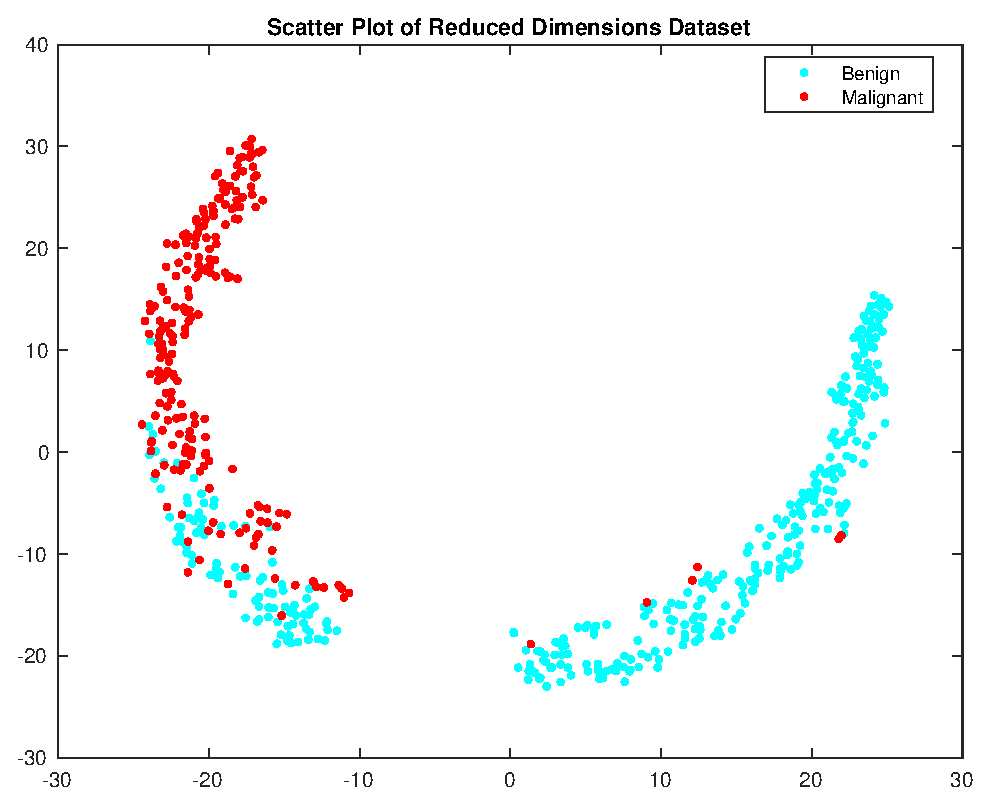
\includegraphics [width=4in]{Project_01.eps}
\begin{par}
As it can be intuitively observed above, the complete dataset was divided into two different categories, however, it appears that it wasn't categorized effectively, as the red responses can also be seen in the majorly blue cluster. Similarly, a few blue responses can also be seen in the majorly blue cluster.
\end{par} \vspace{1em}
\begin{par}
Let us apply k-Means clustering to cluster the dataset in two distinct clusters, then find out the accuracy
\end{par} \vspace{1em}
\begin{tcolorbox}[
    enhanced,
    attach boxed title to top left={xshift=6mm,yshift=-2mm},
    colback=moonstoneblue!20,
    colframe=moonstoneblue,
    colbacktitle=moonstoneblue,
    title=MATLAB Code,
    fonttitle=\bfseries\color{black},
    boxed title style={size=small,colframe=moonstoneblue,sharp corners},
    sharp corners,
    text width=140mm
    ]
\begin{minted}[linenos]{matlab}

% Finding cluster id's using kMeans clustering (2 clusters)
idx = kmeans(reducedDimension,2,'Distance','sqeuclidean');
% Visually comparing the clustering vs the actual responses by plotting
% both of them side by side:
hFig2 = figure(2);
set(hFig2, 'Position', [0 0 1000 500]);
subplot(1,2,1);
gscatter(reducedDimension(:,1), reducedDimension(:,2), txtLabels, 'cr');
hold on;
title('Scatter Plot of Reduced Dimensions Dataset');

subplot(1,2,2);
gscatter(reducedDimension(:,1), reducedDimension(:,2), idx);
hold on;
title('Scatter Plot after k-Means clustering (2 clusters)');

snapnow;
close(hFig2);

\end{minted}
\end{tcolorbox}


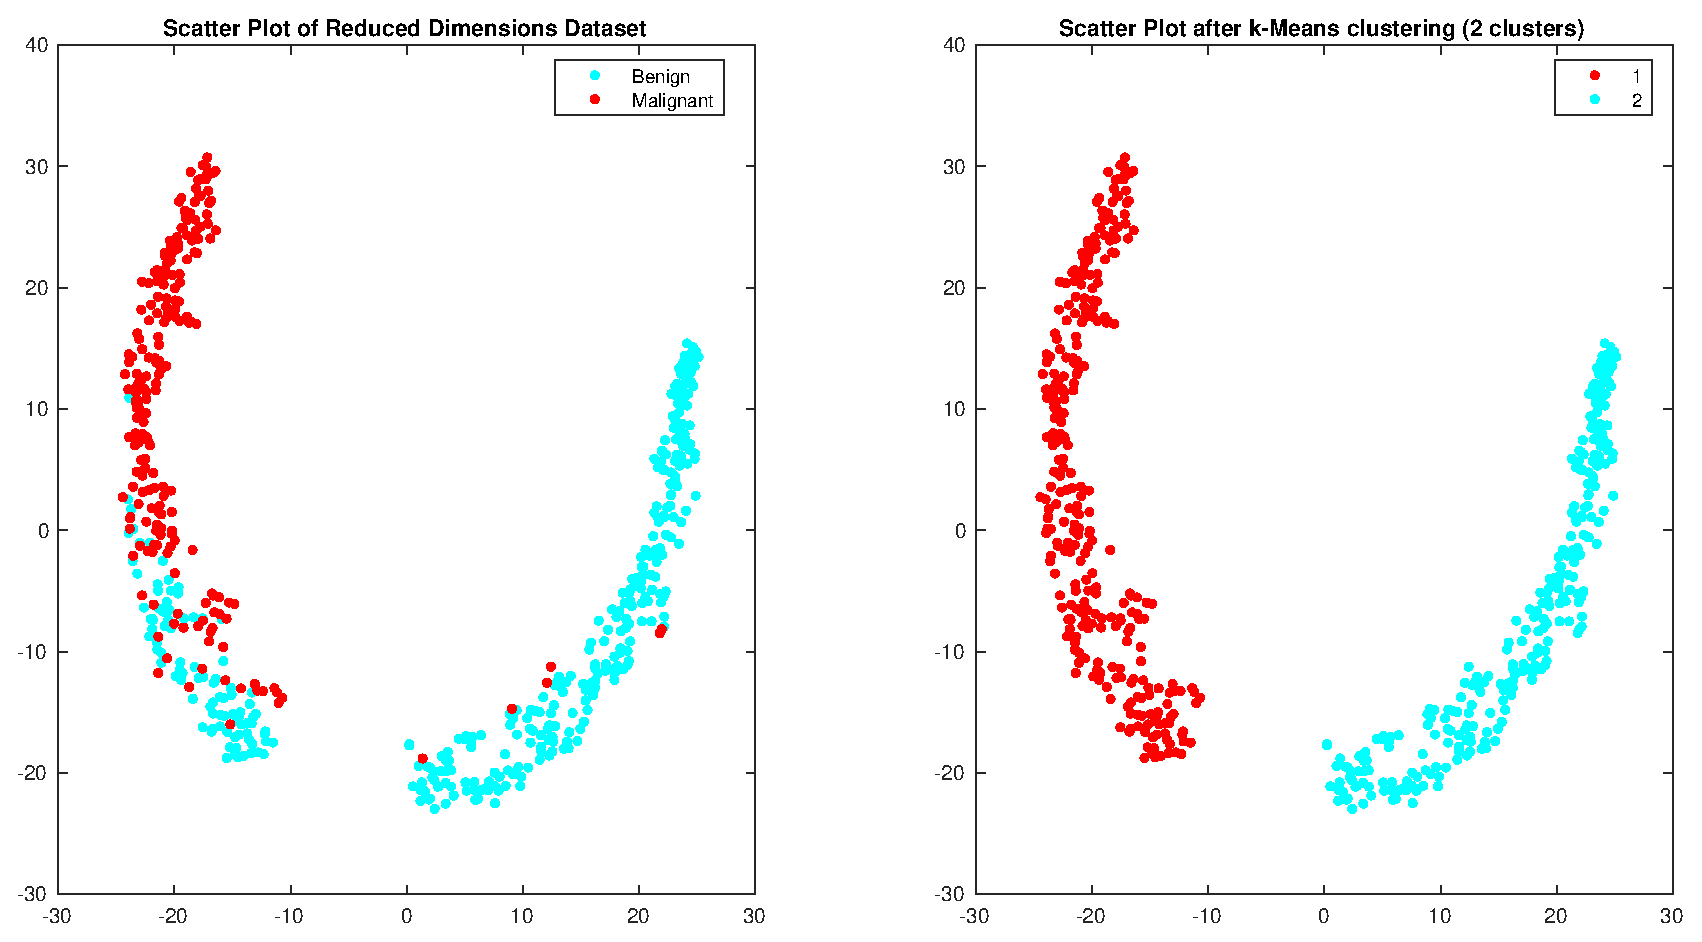
\includegraphics [width=5.8in]{Project_02.eps}
\begin{par}
Let us see the accuracy percentage in this scenario
\end{par} \vspace{1em}
\begin{tcolorbox}[
    enhanced,
    attach boxed title to top left={xshift=6mm,yshift=-2mm},
    colback=moonstoneblue!20,
    colframe=moonstoneblue,
    colbacktitle=moonstoneblue,
    title=MATLAB Code,
    fonttitle=\bfseries\color{black},
    boxed title style={size=small,colframe=moonstoneblue,sharp corners},
    sharp corners,
    text width=140mm
    ]
\begin{minted}[linenos]{matlab}

sum(((idx == 1)*1) == response)/size(response, 1)*100

\end{minted}
\end{tcolorbox}

\begin{tcolorbox}[
    enhanced,
    attach boxed title to top left={xshift=6mm,yshift=-2mm},
    colback=black,
    colframe=grey,
    colbacktitle=grey,
    title=System Output,
    coltext=white,
    fonttitle=\bfseries\color{white},
    boxed title style={size=small,colframe=grey,sharp corners},
    sharp corners,
    text width=100mm,
]
\begin{minted}{text}

ans =

   82.2496

\end{minted}
\end{tcolorbox}


    \begin{par}
Therefore, although the dataset was clearly divided into two distinct clusters, however, the classification was not done as correctly, with the accuracy percent as 82.25\%
\end{par} \vspace{1em}


\section*{7. Summary}

\begin{par}
The summary is shown in the table below, with the best accuracy at the top.
\end{par} \vspace{1em}

\begin{tcolorbox}[
    enhanced,
    attach boxed title to top left={xshift=6mm,yshift=-2mm},
    colback=moonstoneblue!20,
    colframe=moonstoneblue,
    colbacktitle=moonstoneblue,
    title=MATLAB Code,
    fonttitle=\bfseries\color{black},
    boxed title style={size=small,colframe=moonstoneblue,sharp corners},
    sharp corners,
    text width=140mm
    ]
\begin{minted}[linenos]{matlab}

[I,map] = imread('Data/result','png');
imshow(I,map,'InitialMagnification', 50);

\end{minted}
\end{tcolorbox}

% \includegraphics [width=5.8in]{Project_03.eps}


% Please add the following required packages to your document preamble:
% \usepackage{booktabs}
\begin{table}[h]
\begin{tabular}{@{}lll@{}}
\toprule
Model                  & Note                         & Accuracy \\ \midrule
Linear Regression      & Selected Features            & 97.03    \\
k Nearest Neighbor (5) & 10-Fold Cross Validation     & 97.01    \\
k Nearest Neighbor (5) & Basic                        & 96.04    \\
ECOC                   & Basic                        & 96.04    \\
Linear Regression      & 10-Fold \& Feature Selection & 95.61    \\
k Nearest Neighbor (5) & Selected Features            & 94.96    \\
Linear Regression      & 10-Fold Cross Validation     & 92.62    \\
Linear Regression      & Basic                        & 92.08    \\
ECOC                   & 10-Fold Cross Validation     & 91.39    \\
Unsupervised Learning  & tSNE                         & 82.25    \\ \bottomrule
\end{tabular}
\end{table}


\begin{par}
Therefore, linear regression done after feature selection, which was then tested on the test-data gave us the best accuracy, where as reducing the dimensions of the dataset to two using tSNE, followed by k-Means clustering (2 clusters) gave us the worst accuracy amongst all the methodologies used.
\end{par} \vspace{1em}



\end{document}
    
